\section{Auswertung}
\label{sec:Auswertung}
Im folgenden wird die Stabilitätsbedingung des Lasers überprüft und die TEM-Moden verglichen. Außerdem wird die Polarisation und die Wellenlänge des Lasers bestimmt.

\subsection{Stabilitätsbedingung}
Gemäß Formel \ref{eqn:Stab} wird die Stabilitätsbedingung für die beiden getroffenen Spiegelkonstellationen im folgenden untersucht. In Abbildung \ref{fig:stabi} ist das Produkt der Spiegelparameter in Abhängikeit der Resonatorlänge aufgetragen.
\begin{figure}
  \centering
  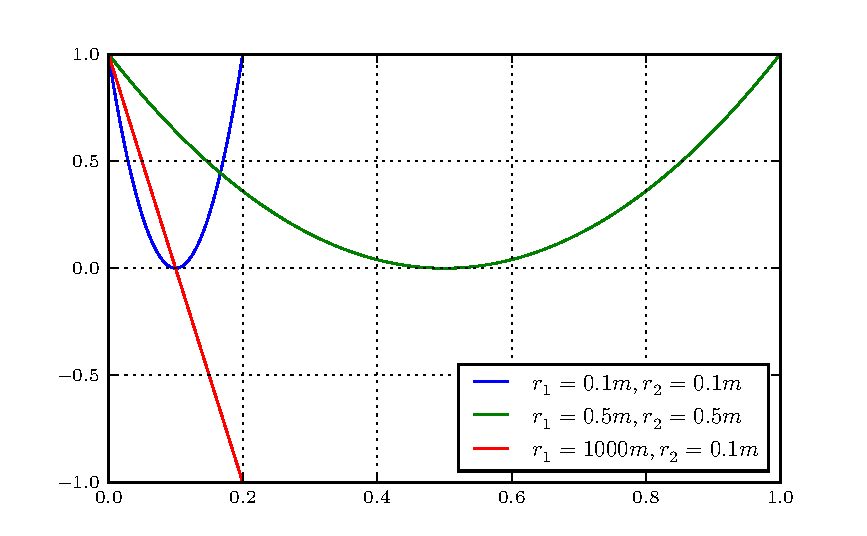
\includegraphics[width=\textwidth]{Stabilisationsparameter.pdf}
  \caption{Stabilitätsbedingung des Resonators}
  \label{fig:stabi}
\end{figure}
Aus dem Diagramm kann abgelesen werden, dass bei Verwendung zweier Spiegel mit einem Krümmungsradius von
\begin{equation}
  r_1 = 1400 \, \text{mm}
  \label{eqn:rad1}
\end{equation}
die maximal zu erwartende Reichweite
\begin{equation}
  R_\text{1 max} = 2.8 \, \text{m}
  \label{eqn:rmax1}
\end{equation}
ist. In diesem Bereich läuft der Laser stabil und es kann ein Laserstrahl detektiert werden. Dies kann jedoch im Experiment nicht verifiziert werden, da die Schiene auf welchen die Resonatorspiegel sitzen zu kurz ist. Die maximale Reichweite muss demnach größer als 2,2 m sein. Bei der Verwendung von einem geraden Spiegel und einem Spiegel mit Krümmungsradius $r_1$ ergibt sich eine theoretische Reichweite von
\begin{equation}
  R_\text{2 max} = 1.4 \, \text{m} \ .
  \label{eqn:rmax2}
\end{equation}
Diese Reichweite wird verifiziert indem die Intensität der gemessenen Laserstrahlung von 100 $\mu$A bei einem Resonatorabstand von 1.40 m auf 2 $\mu$A abfällt und der Laserstahl für weitere Reichweiten nicht weiter zu detektieren ist.

\subsection{TEM}
Da die Intensität der Laserstrahlung selbst nicht gemessen werden kann, wird stattdessen ein Photostrom einer Diode gemessen. Dieser ist proportional zur Intensität. Auf die Ströme, welche in Tabelle \ref{tab:tem} aufgetragen sind, wird in der Auswertung noch weiter eingegangenen.
\begin{table}
  \centering
  \caption{Diodenstrom in Abhängigkeit des Abstandes}
  \begin{tabular}{c|c c}
     \toprule
     Abstand / mm & TEM$_{00}$ I / µA & TEM$_{10}$ I / µA \\
     \midrule
     0		& 0.058		& 0.041	\\
     1		& 0.112		& 0.078	\\
     2		& 0.199		& 0.142	\\
     3		& 0.332		& 0.166	\\
     4		& 0.458		& 0.204	\\
     5		& 0.623		& 0.298	\\
     6		& 1.187		& 0.367	\\
     7		& 1.221		& 0.286	\\
     8		& 2.120		& 0.384	\\
     9		& 2.332		& 0.233	\\
     10		& 3.140		& 0.220	\\
     11		& 3.165		& 0.076	\\
     12		& 3.954		& 0.048	\\
     13		& 4.195		& 0.010	\\
     14		& 4.222		& 0.024	\\
     15		& 4.408		& 0.100	\\
     16		& 5.006		& 0.204	\\
     17		& 4.207		& 0.387	\\
     18		& 3.644		& 0.502	\\
     19		& 2.903		& 0.562	\\
     20		& 2.323		& 0.601	\\
     21		& 1.580		& 0.499	\\
     22		& 1.352		& 0.760	\\
     23		& 1.172		& 0.701	\\
     24		& 0.904		& 0.603	\\
     25		& 0.673		& 0.512	\\
     26		& 0.522		& 0.422	\\
     27		& 0.220		& 0.244	\\
     28		& 0.186		& 0.249	\\
     29		& 0.143		& 0.200	\\
     30		& 0.062		& 0.070	\\
     31		& 0.053		& 0.059	\\
     \bottomrule
  \end{tabular}
  \label{tab:tem}
\end{table}
Im folgenden wird geprüft, ob die Intensitäten entsprechend von den Hermitpolynomen bzw. Laguerre-Polynomen abhängig sind.
\subsubsection{TEM$_\text{00}$}
Die niedrigste Mode, welche gleichzeitig die höchste Intensität aufweist, wird ohne eine Modenblende erzeugt. Die mittels Photodiode gemessenen Ströme der TEM$_{00}$ sind in Tabelle \ref{tab:tem} aufgeführt und in Abbildung \ref{fig:TEM00} abgebildet. Dabei wurde die Auslenkung der Diode gegen den Photostrom aufgetragen.
\begin{figure}
  \centering
  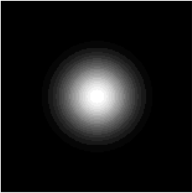
\includegraphics[width=\textwidth]{TEM00.pdf}
  \caption{Diodenstrom der ersten Mode in Abhängigkeit von der Auslenkung der Diode}
  \label{fig:TEM00}
\end{figure}
Anhand von den Photoströmen wird entsprechend der Formel \ref{eqn:Grund} ein Fit der Form
\begin{equation}
  I(x) = I_0 \cdot e^{- \frac{(x-\bar{x})^2}{\omega^2} }
  \label{eqn:gausian}
\end{equation}
durch die Messwerte gelegt. Wobei $I_0$ der Amplitude, $\bar{x}$ dem Mittelwert und $\omega$ der Standardabweichung der Gaußfunktion entspricht. Dabei ist explizit eingegangen, dass das Hermitpolynom 0. Ordnung
\begin{equation}
  H_0 = 1
  \label{}
\end{equation}
ist. Der Fit dient zum Vergleich mit dem Theoriewert und der Überprüfung, ob die Intensität von den Laguerre-Polynomen abhängig ist. Es ergeben sich Fitparameter von
\begin{eqnarray}
  I_0 =& (\num{4.53 +- 0.08})	\\
  \bar{x} =& (\num{9.9 +- 0.2})	\\
  \omega =& (\num{14.6 +-0.1})
  \label{eqn:coef}
\end{eqnarray}
\subsubsection{TEM$_\text{10}$}
Zum erzeugen der ersten Mode wird ein Wolframdraht als Modenblende in den Strahlengang gestellt und solange ausjustiert, bis der Strahlengang sich in zwei Punkte aufspaltet. Die mittels der Photodiode gemessenen Ströme in Abhängikeit der Auslenkung sind in Tabelle \ref{tab:tem} aufgetragen und in Abbildung \ref{fig:TEM10} dargestellt.
\begin{figure}
  \centering
  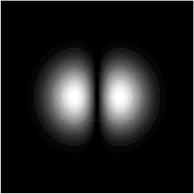
\includegraphics[width=\textwidth]{TEM10.pdf}
  \caption{Diodenstrom der ersten Mode in Abhängigkeit von der Auslenkung der Diode}
  \label{fig:TEM10}
\end{figure}
Das zweite Hermitpolynom lautet
\begin{equation}
  H_2 = 4x^2 - 2
  \label{eqn:Herm}
\end{equation}
Daraus ergibt sich der Fit der Form
\begin{equation}
  I(x) = I_0 \cdot 8 \frac{\left( x - \bar{x} \right)}{\omega^2} \cdot e^{-2 \frac{\left( x - \bar{x} \right)^2}{\omega^2}}
  \label{eqn:TEM10}
\end{equation}
welcher durch die Messwerte gelegt wird, um diese mit der theoretischen Vorhersage zu vergleichen. Die Fitparameter sind
\begin{eqnarray}
  I_0 =& \num{0.36 +- 0.03}	\\
  \bar{x} =& \num{10.0 +- 0.5} \\
  \omega =& \num{14.1 +- 0.4}
\end{eqnarray}

\subsection{Polarisation der Laserstrahlung}
Die Intensität in Abhängigkeit der Ausrichtung des Polarisationsfilters ist in Tabelle \ref{tab:Pol} und in Abbildung \ref{fig:Pol} aufgetragen.
\begin{table}
  \centering
  \caption{Intensität in Abhängigkeit des Polarisationswinkels}
  \begin{tabular}{c c | c c}
    \toprule
    $\varphi$ / Grad & Intensität / µA & $\varphi$ / Grad & Intensität /µA \\
    \midrule
	0	& 44.3	& 10	& 23.6	\\
	20	& 9.7	& 30	& 0.7	\\
	40	& 2.8	& 50	& 13.8	\\
	60	& 36.0	& 70	& 55.2	\\
	80	& 89.0	& 90	& 143.0	\\
	100	& 145.0	& 110	& 186.7	\\
	120	& 181.5	& 130	& 205.0	\\
	140	& 170.2	& 150	& 150.6	\\
	160	& 122.9	& 170	& 66.0	\\
	180	& 48.3	& 190	& 25.1	\\
	200	& 7.9	& 210	& 0.7	\\
	220	& 1.8	& 230	& 13.6	\\
	240	& 27.0	& 250	& 52.2	\\
	260	& 85.1	& 270	& 99.2	\\
	280	& 163.2	& 290	& 178.9	\\
	300	& 195.4	& 310	& 195.3	\\
	320	& 166.6	& 330	& 149.5	\\
	340	& 133.3 & 350	& 94.1	\\
	360	& 43.2	\\
    \bottomrule
  \end{tabular}
  \label{tab:Pol}
\end{table}
Dabei wird ein Fit der Form
\begin{equation}
  I(\varphi) = A_0 \cdot \sin(\omega x + \mu) + d
  \label{eqn:pfit}
\end{equation}
durch die Messwerte gelegt.
\begin{figure}
  \centering
  \includegraphics[width=\textwidth]{Polar.pdf}
  \caption{Intensität in Abhängigkeit des Polarisationswinkels}
  \label{fig:Pol}
\end{figure}
Anhand des Graphens wird in der Disskussion eine Aussage über die Polarisation getroffen.
\subsection{Wellenlänge des Lasers}
Zur Bestimmung der Wellenlänge des Lasers wird ein Gitter der Gitterkonstanten
\begin{equation}
  G = 10^5 \, \frac{1}{\text{m}}
  \label{eqn:constg}
\end{equation}
in den Laserstrahl gestellt. Der Abstand von dem Gitter bis zum Schirm beträgt
\begin{equation}
  L = 1.741 \, \text{m} \ .
  \label{eqn:K}
\end{equation}
Die gemessenen Abstände $a$ der einzelen Nebenmaxima vom Hauptmaximum sind in Tabelle \ref{tab:max} aufgetragen.
\begin{table}
  \centering
  \begin{tabular}{c c c}
    \toprule
    n-tes Maximum & $a_\text{links}$ $\frac{1}{\text{cm}}$ & $a_\text{rechts}$ $\frac{1}{\text{cm}}$ \\
    \midrule
	1 & 11.2 & 11.0 \\
	2 & 22.5 & 22.2 \\
	3 & 34.3 & 33.8 \\
    \bottomrule
  \end{tabular}
  \caption{Abstand der Nebenmaxima vom Hauptmaximum}
  \label{tab:max}
\end{table}
Aus den Abständen lässt sich anhand von Formel \ref{eqn:lambda} die Wellenlänge des Lasers berechnen. Sie beträgt
\begin{equation}
  \lambda = (\num{652 +- 8}) \, \text{nm} \ .
\end{equation}
